%%%%%%%%%%%%%%%%%%%%%%%%%%%%%%%%%%%%%%%%%
% FRI Data Science_report LaTeX Template
% Version 1.0 (28/1/2020)
% 
% Jure Demšar (jure.demsar@fri.uni-lj.si)
%
% Based on MicromouseSymp article template by:
% Mathias Legrand (legrand.mathias@gmail.com) 
% With extensive modifications by:
% Antonio Valente (antonio.luis.valente@gmail.com)
%
% License:
% CC BY-NC-SA 3.0 (http://creativecommons.org/licenses/by-nc-sa/3.0/)
%
%%%%%%%%%%%%%%%%%%%%%%%%%%%%%%%%%%%%%%%%%


%----------------------------------------------------------------------------------------
%	PACKAGES AND OTHER DOCUMENT CONFIGURATIONS
%----------------------------------------------------------------------------------------
\documentclass[fleqn,moreauthors,10pt]{ds_report}
\usepackage[english]{babel}

\graphicspath{{fig/}}




%----------------------------------------------------------------------------------------
%	ARTICLE INFORMATION
%----------------------------------------------------------------------------------------

% Header
\JournalInfo{FRI Natural language processing course 2023}

% Interim or final report
\Archive{Project report} 
%\Archive{Final report} 

% Article title
\PaperTitle{An Automatic Movie Summary Generator} 

% Authors (student competitors) and their info
\Authors{Luka Pavićević, Andrija Stanišić, Stefanela Stevanović}

% Advisors
\affiliation{\textit{Advisors: Slavko Žitnik, Aleš Žagar}}

% Keywords
\Keywords{Movie script summarization, Latent Semantic Analysis, Text-To-Text
Transfer Transformer}
\newcommand{\keywordname}{Keywords}


%----------------------------------------------------------------------------------------
%	ABSTRACT
%----------------------------------------------------------------------------------------

\Abstract{
This project aims to automate the summarization of movie scripts using Natural Language Processing (NLP) techniques. We explore a baseline approach using Latent Semantic Analysis (LSA) and a main approach utilizing the T5 (Text-To-Text Transfer Transformer) model. The generated summaries provide movie enthusiasts with concise information about a movie's plot, characters, and key events. While the results are promising, there is room for improvement in terms of coherence and accuracy. Automating script summarization using NLP offers a time-saving solution for movie enthusiasts, with the potential for further enhancement and improved user experience in movie exploration.
}

%----------------------------------------------------------------------------------------

\begin{document}

% Makes all text pages the same height
\flushbottom 

% Print the title and abstract box
\maketitle 

% Removes page numbering from the first page
\thispagestyle{empty} 

%----------------------------------------------------------------------------------------
%	ARTICLE CONTENTS
%----------------------------------------------------------------------------------------

\section*{Introduction}

In today's fast-paced world, where an overwhelming number of movies are released each year, staying updated with the latest releases can be a challenge for audiences. To make informed decisions about which movies to watch, many people turn to summaries or synopses. However, manually summarizing lengthy movie scripts can be a time-consuming and difficult task.

Fortunately, Natural Language Processing (NLP) offers a solution. By leveraging NLP techniques, we can automate the process of summarizing movie scripts, saving valuable time and effort.

This project aims to develop a solution that effectively summarizes movie scripts into concise and informative synopses using NLP. By providing movie enthusiasts with a convenient and efficient way to grasp a movie's plot, characters, and significant events, our solution aims to assist them in making informed decisions about which movies to watch.


\section*{Related works}

One of the related works in text summarization is the work by Aleš Žagar and Marko  Robnik-Šikonja \cite{zagar2022}, who explored the use of various summarization approaches, including neural models, to produce short summaries from larger texts. In their work, they addressed the problem of selecting the most appropriate summarization model for a given text, and proposed a solution that uses a neural metamodel to automate the selection process based on the input document's representation. This work presents an innovative approach to text summarization, particularly in addressing the issue of model selection, which is important in ensuring the quality of generated summaries.

The article \cite{APARICIO20167} discusses the performance of generic text summarization algorithms on movies and documentaries, using extracts from news articles produced by reference models of extractive summarization. The study aims to evaluate the quality of automatic summaries produced for movies and documentaries, using well-known behaviors of news articles as a reference. Six text-based summarization approaches were used: Maximal Marginal Relevance (MMR), LexRank, Latent Semantic Analysis (LSA), Support sets, Key Phrase-based Centrality (KP-Centrality), and TextRank. The study found that LexRank and Support Sets had the best performance on movies of all the mentioned aproaches.

The paper \cite{DHARANIYA2023102150} proposes an ensemble deep learning model for generating movie scripts, which means that multiple models are combined to improve the accuracy and robustness of the system.  The model uses the Ensemble-based Movie Scrip Generation (EMCG), where the Optimized hybrid script generation process using ensemble learning is performed by Bi-LSTM, GPT3, and GPT Neo X models, where the parameters of deep learning algorithms are optimized using the AI-CMO algorithm.

\section*{Corpus}

For our project, we gathered data from various sources including scripts from IMSDb, summaries from Metacritic (MC) and Rotten Tomatoes (RT), as well as subtitles and summaries from Subslikescript (SLS). In addition to that, we also collected some other available data such as movie genres and year of release. Initially, we merged the IMSDb scripts with all other available data to create the first dataset. However, some of the scripts did not have corresponding summaries or subtitles. Therefore, we merged these scripts with whatever data was available for them. In the process of data cleaning, we identified that some of the subtitles contained an unreasonably low number of sentences, some having as few as one. As a result, we removed all subtitles containing less than 100 sentences. This left us with the following data set:
\begin{itemize}
  \item IMSDb Scripts: 943 entries
  \item Subslikescript Subtitles: 772 entries
  \item Subslikescript Summaries: 785 entries
  \item Metacritic Summaries: 835 entries
  \item Rotten Tomatoes Summaries: 781 entries
\end{itemize}

For this dataset we performed the corpus analysis, that is shown in table 1. 

\begin{table}[h]
\caption{Average, minimum and maximum number of sentences, words and TTR for the data in the first data set, collected from different sources.}
\begin{center}
\begin{tabular}{c|c|ccc}
  & DATA & AVG & MIN &  MAX\\
 \hline
  & IMSDb Scripts &  2807&  334  & 5345\\ 
  & SLS Subtitles &  1505& 121 & 11077 \\
Sentences & SLS Summaries&  4 & 1 & 22 \\
& MC Summaries &  2 & 1 & 12\\
& RT Summaries &  3 & 1 & 7 \\
 \hline
  & IMSDb Scripts &  29421& 4302  & 64311\\ 
  & SLS Subtitles &  11660& 718 & 49988 \\
Words & SLS Summaries&  123 & 12 & 616 \\
& MC Summaries &  64 & 10 & 320\\
& RT Summaries &  82 & 7 & 123 \\
\hline
  & IMSDb Scripts &  0.143&  0.071  & 0.312\\ 
  & SLS Subtitles &  0.157& 0.002 & 0.422 \\
TTR & SLS Summaries&  0.696 & 0.471 & 1.000 \\
& MC Summaries &  0.828 & 0.534 & 1.000\\
& RT Summaries &  0.757 & 0.600 & 1.000 \\
\end{tabular}
\label{tab1}
\end{center}
\end{table}

\begin{figure}[h]
\begin{center}
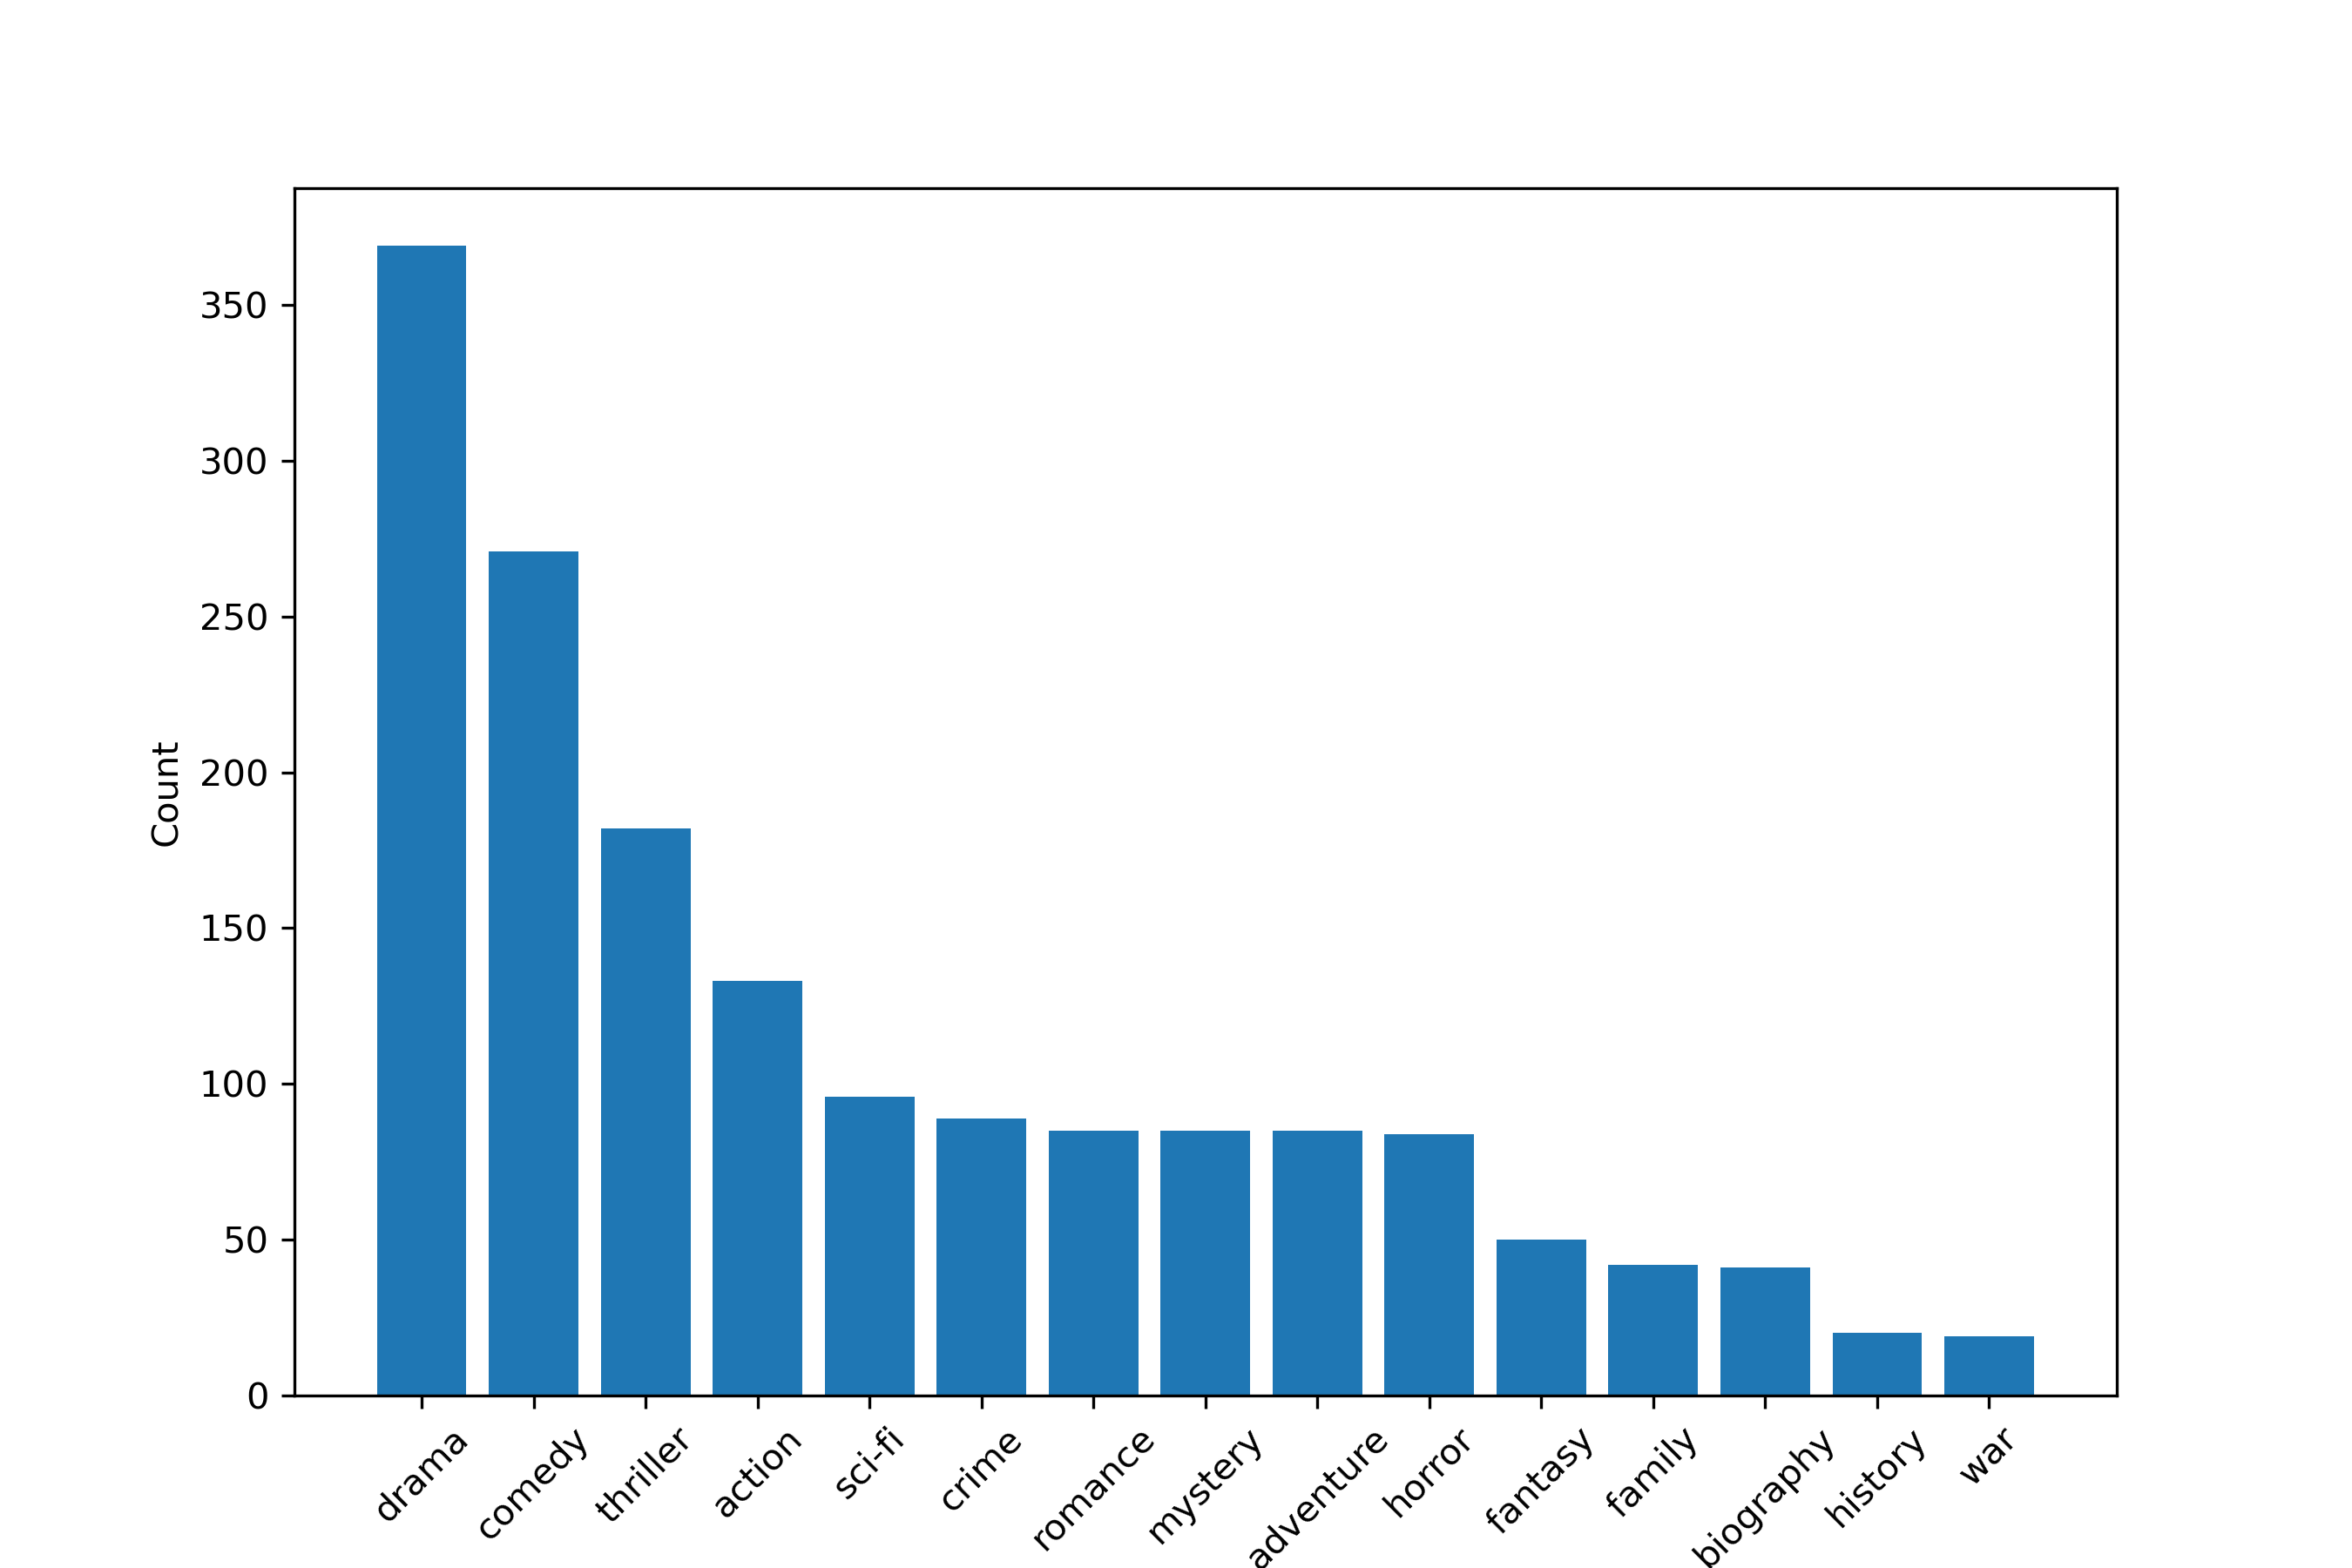
\includegraphics[width=1.0\columnwidth]{movie_genres.png}
\end{center}
\caption{Top 15 most common movie genres in our first data set. The most prevalent genre is drama, followed by comedy and thriller.}
\label{fig1}
\end{figure}

For our analysis, we utilized genre data available from Rotten Tomatoes and Metacritic. As each movie can belong to multiple genres, we performed an intersection between the genres from these two sites to obtain a more concise and accurate genre description for each movie. The objective was to avoid having too many genres associated with the same movie. Next, we counted the occurrence of each genre within the intersected movie genres, and plotted the 15 most common genres in Figure 1.



\section*{Baseline aproach}

As a baseline approach to summarizing the movie scripts in this project, we employ Latent Semantic Analysis (LSA). 

LSA is a popular text summarization technique that uses singular value decomposition (SVD) to reduce the dimensionality of a document-term matrix and capture the underlying semantic structure of the text. The model assumes that words with similar meanings will appear in similar contexts and can be grouped together.

To use the LSA model for text summarization, we split the movie scripts into scenes and preprocess the scene text by converting it to lowercase, removing non-alphanumeric characters from each sentence. We then use the Sumy library to tokenize the scene text and prepare it for input into the LSA model.

The LSA model identifies the most important sentences in a document based on their semantic similarity to other sentences. We use the LsaSummarizer module from Sumy to generate a summary of each scene, with a target of two sentences per scene.

After generating the summaries using LSA, we evaluate their quality using the ROUGE metric. ROUGE is a commonly used metric for evaluating text summarization models that measures the overlap between the generated summary and the reference summary. ROUGE provides multiple scores such as ROUGE-1, ROUGE-2, and ROUGE-L.

ROUGE-1 measures the overlap of unigrams (single words) between the generated and reference summaries. ROUGE-2 measures the overlap of bigrams (pairs of adjacent words) between the generated and reference summaries. ROUGE-L is a variant that computes the longest common subsequence between the generated and reference summaries, which can handle paraphrasing and word order differences.

The Fig. 2. shows the average ROUGE scores for each of the three metrics for each reference summary. We achieved decent scores for ROUGE-1 and ROUGE-L, bearing in mind that this is only a baseline model.  However, our model struggled to capture longer, more complex phrases and sentences, as reflected in the low score for ROUGE-2.

We believe that the poor performance on ROUGE-2 may be due to the fact that LSA is a bag-of-words model and does not capture word order or phrase structure. Additionally, the model may struggle with more complex sentences that contain multiple clauses or dependent phrases. Despite these limitations, our baseline approach with LSA provides a reasonable starting point for summarizing movie scripts and could be improved with further optimization and fine-tuning. 

\begin{figure}[h]
\begin{center}
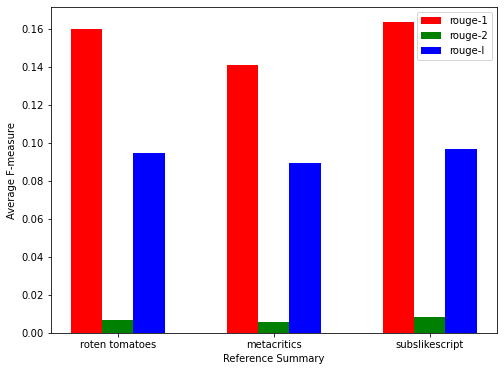
\includegraphics[width=1.0\columnwidth]{rouge_scores.png}
\end{center}
\caption{ROUGE Scores by Reference Summary}
\label{fig1}
\end{figure}

\section*{The main aproach}

The main model used in this project is the T5 (Text-To-Text Transfer Transformer) model. T5 is a Transformer architecture developed for various natural language processing tasks, including text summarization.

The T5 model consists of an encoder-decoder architecture based on the Transformer model. The encoder part of the model processes the input text and obtains its representation. The decoder part of the model then uses this representation to generate the output summary.

To use the T5 model, we first initialize a Tokenizer object. The Tokenizer is used to convert text into a sequence of tokens, which is required as input for the model.
For text summarization, we need to define the maximum length of the input and output sequences expected by the model. Additionally, we can add an appropriate prefix to the input text to clearly indicate to the model that the task is summarization.
Afterward, the data is preprocessed to prepare it for input to the model. The input text is tokenized and encoded, and the target summary is also tokenized and encoded.

The training-test set split was intentionally performed to include 43 well-known movies in the test set. 
After training the model, we use it to generate summaries. This can be achieved by using a pipeline approach, where the input scripts from the test set are passed to the model, and the generated summaries are obtained as the result.

Finally, to evaluate the generated summaries, we employ the BERTScore metric. BERTScore is a metric based on the BERT (Bidirectional Encoder Representations from Transformers) model, which measures the similarity between generated and reference texts. This metric takes into account the semantic similarity and contextual word representation when evaluating the generated summaries.

We calculated precision, recall, and F1 score for each generated summary and obtained the following results: precision = 0.839, recall = 0.819, and F1 score = 0.829. These metrics provide an objective measure of the generated summaries' quality compared to the reference summaries.

In addition to the BERTScore evaluation, the personal analysis was conducted to provide further insights. It was observed that the generated summaries often focus on family relationships, there are cases of repetitive word usage without necessity, and vast majority of summaries begins with the name of the main character. Furthermore, it was noticed that the generated summaries often emphasize certain characters as being the only or the first ones to experience certain events.

Below are several examples of summaries generated by the model, accompanied by comments:

\begin{enumerate}[noitemsep]
	\item     Prestige:
 
    \textit{Robert Angier (Borden) is a magician and magician who has a reputation as an amateur magician. He's a young magician and a writer who's been a fan of the magician's magic.}
    
    The summary captures certain elements but lacks coherence and clarity. It repeats phrases and fails to provide a concise overview of the movie.

    \item Inglorious Basterds:
    
    \textit{The French Farmer, a former Nazi colonel, is a slain rat who has been killed by the Nazis in the past year. He is the only one to be killed by a Nazi rat, who has escaped from the Nazi army. The rat's father, the Napoleon, is the first to be murdered by the Nazis in the world.}
    
    The summary contains some movie elements but includes incorrect information and lacks coherence. The mention of a "Nazi rat" and a character named "the Napoleon" is confusing and does not accurately represent the movie's plot.

    \item Joker:
    \textit{Joker is a snub-nose, a man who has a brain injury and a lack of empathy for his family. He's a big fan of comedy, but he is able to make a difference in his life. Joker's mother, whose daughter, is an adolescent, tries to get her back on the streets of Gotham.}
    
    The summary touches on several aspects of the movie but lacks coherence and clarity. The mention of a "snub-nose" is not accurate.

    \item Memento:
    \textit{Leonard, a late model, has a tattoo of a polaroid that he's known for. He tries to find a way to make his life easier, but he can't make any new memories.}
    
    The summary provides a good understanding of the movie's premise, but lacks the complexity of the main character's condition.

    \item Silence of the Lambs:
    
    \textit{Dr. Lecter, a psychiatrist, is a psychiatric therapist and a psychotherapist. He is an adolescent psychopath who has a history of psychosis. The psychiatrist, who is based in the city of Split City, is the first person to have a mental illness.}
    
    The summary correctly acknowledges Dr. Lecter's mental illness and his expertise as a psychiatrist. However, it is important to note that he is not the first person with such a condition, and also that he is not an \textit{adolescent}.
\end{enumerate}

\section*{Conclusion}

In this project, we aimed to automate the process of summarizing movie scripts using Natural Language Processing techniques. We explored different approaches, starting with a baseline model based on Latent Semantic Analysis (LSA), and then implementing the main approach using the T5 model. Our results showed a decent quality of summaries generated by both baseline and the main model.

However, we also identified certain limitations in the generated summaries, such as the repetition of phrases, lack of coherence, and occasional inaccuracies. These areas could be further improved through model optimization and fine-tuning. Additionally, a personal analysis revealed certain patterns in the generated summaries, such as a focus on family relationships and the emphasis on specific characters.

Despite these limitations, the automated summarization of movie scripts using NLP techniques provides a valuable tool for movie enthusiasts. It allows them to quickly grasp the plot, characters, and key events of a movie, aiding in the decision-making process when choosing which movies to watch.

Overall, this project demonstrates the potential of NLP in automating the task of movie script summarization. Future work could involve refining the models, addressing the identified limitations, and exploring other NLP techniques to enhance the accuracy and coherence of the generated summaries. The development of such solutions can greatly benefit movie lovers by providing them with a time-efficient and informative way to explore a vast array of movies.
%----------------------------------------------------------------------------------------
%	REFERENCE LIST
%----------------------------------------------------------------------------------------
\bibliographystyle{unsrt}
\bibliography{report}


\end{document}